%%%% Various options for document class.
%\documentclass[usenatbib, a4paper]{preprint}
\documentclass[preprint, a4paper, 11pt]{aastex}
%%\documentclass[twocolum]{revtex4}
%%\documentclass{report}
%%\documentclass[useAMS,usenatbib, onecolumn]{mn2ejm}

%\usepackage{psfig,morefloats,url}
%use preprint2 for 2 columns paper.

%% declare any packages used
\usepackage{graphicx}
\usepackage{natbib}
\usepackage{graphicx}
\usepackage{color}
\usepackage{pdfpages}
\usepackage{appendix}
%\usepackage{epsfig}
%\usepackage[dvips]{color}
%\usepackage{aabib}


%\marginparwidth = 25pt
\citestyle{aa}
\addtolength{\topmargin}{-.5in}
%% This command added as margins are wrong in mn2e, it appears. 
%% Not needed for other classes

%% This is the end of the preamble.  Indicate the beginning of the
%% paper itself with \begin{document}.


%%%%%%%%%%%%%%%%%%%%%%%%%%%%%%%%%%%%%%

\begin{document}
%% define bibstyle and other definitions
\bibliographystyle{aabib}
%% renew commands
\renewcommand{\labelitemi}{$-$}
\def\la{Ly-$\alpha$ }
\def\py{\textsc{Python} }
\def\civ{C~\textsc{iv} }
\def\araa{ARAA}
\def\nat{Nature}
\def\apjl{ApJ Letters}
\def\aapr{AAPR}
\def\ssr{SSR}
\def\apj{ApJ}
\def\pasp{PASP}
\def\aap{A\&A}
\def\mnras{MNRAS}
\def\aj{AJ}
\def\rmxaa{RMXAA}

%%%%%%%%%%%%%%%%%%%%%%%%%%%%%%%%%%%%%%
%
%          TITLE AND AUTHORS
%
%%%%%%%%%%%%%%%%%%%%%%%%%%%%%%%%%%%%%%%


\title{The Disk Wind Contribution to the Optical Spectra of Cataclysmic Variables}
\author{J. H.
  Matthews, C. Knigge, K. S. Long, S. A. Sim \& N. Higginbottom}
%%\altaffiltext{1}{School of Physics \& Astronomy, University of Southampton,
  %%Southampton, SO17 1BJ, UK}


%%%%%%%%%%%%%%%%%%%%%%%%%%%%%%%%%%%%%%
%
%          ABSTRACT
%
%%%%%%%%%%%%%%%%%%%%%%%%%%%%%%%%%%%%%%%




\begin{abstract}
High-State non-magnetic Cataclysmic Variable systems (CVs) exhibit strong emission in Hydrogen \& Helium 
optical recombination lines. Here we present results obtained by encorporating a macro atom treatment into
our Monte Carlo radiative transfer code originally used
to model UV resonance lines in CVs, \py. Our benchmark CV model is capable of producing
all of the notable optical lines (e.g. He II 4686, H${\alpha}$, He I), as well as
enchanced emission in the Ly-$\alpha$ and He II $1640$ UV lines.
In addition, the improved treatment of recombination means that the bound-free continuum
emission is sufficient to mask the so-called `Balmer jump' photoabsorption edge, 
suggesting a potential solution to a longstanding problem. 
\end{abstract}

\maketitle



%%%%%%%%%%%%%%%%%%%%%%%%%%%%%%%%%%%%%%
%
%          INTRODUCTION
%
%%%%%%%%%%%%%%%%%%%%%%%%%%%%%%%%%%%%%%%

\section{Introduction} 

Non-magnetic Cataclysmic Variables (CVs), are systems in which a white dwarf accretes matter from a donor star
through Roche-lobe overflow onto an accretion disk. It has been shown that the spectra of high state CVs
exhibit absorption features believed to be caused by an outflow, potentially line-driven,
rising from the accretion disk \citep{cordova1982}. 
The ultraviolet spectra of CVs, in particular, exhibit P-Cygni like profiles in resonance lines such as 
NV, OVI and, most commonly, CIV. This hints at the possibility of the wind being line driven, 
as these resonance lines must experience a line force if they are photoionised by a disk or other photon source
close to the centre of the system.


Multiple attempts have been made to model UV wind spectra by treating the wind
as a biconical flow arising from the accretion disk, and conducting radiative transfer simulations to attempt
to reproduce the resonance lines that appear in the spectra. The first generation of models
applied knowledge gleaned from stellar wind modeling to the problem (Mauche \& Raymond
1987; Drew 1987; Vitello \& Shlosman 1988), showing that mass loss rates of $\sim10\%$ of the accretion rate
 were required to produce the required line strengths.
Shlosman \& Vitello (1993; hereafter SV93) describe a radiative transfer code which first computes
an ionization structure based on constant wind temperature, and then used the Sobolev approximation
for line transfer.

A brief Review of optical spectra, and the problems relating to the Balemr Jump will go here.


\newpage
%%%%%%%%%%%%%%%%%%%%%%%%%%%%%%%%%%%%%%
%
%          THE MODEL
%
%%%%%%%%%%%%%%%%%%%%%%%%%%%%%%%%%%%%%%%

\section{A Biconical Wind CV Model}

What motivates this model. Literature. 

\subsection{Description of Model: Geometry and Kinematics}
\begin{figure}
\centering
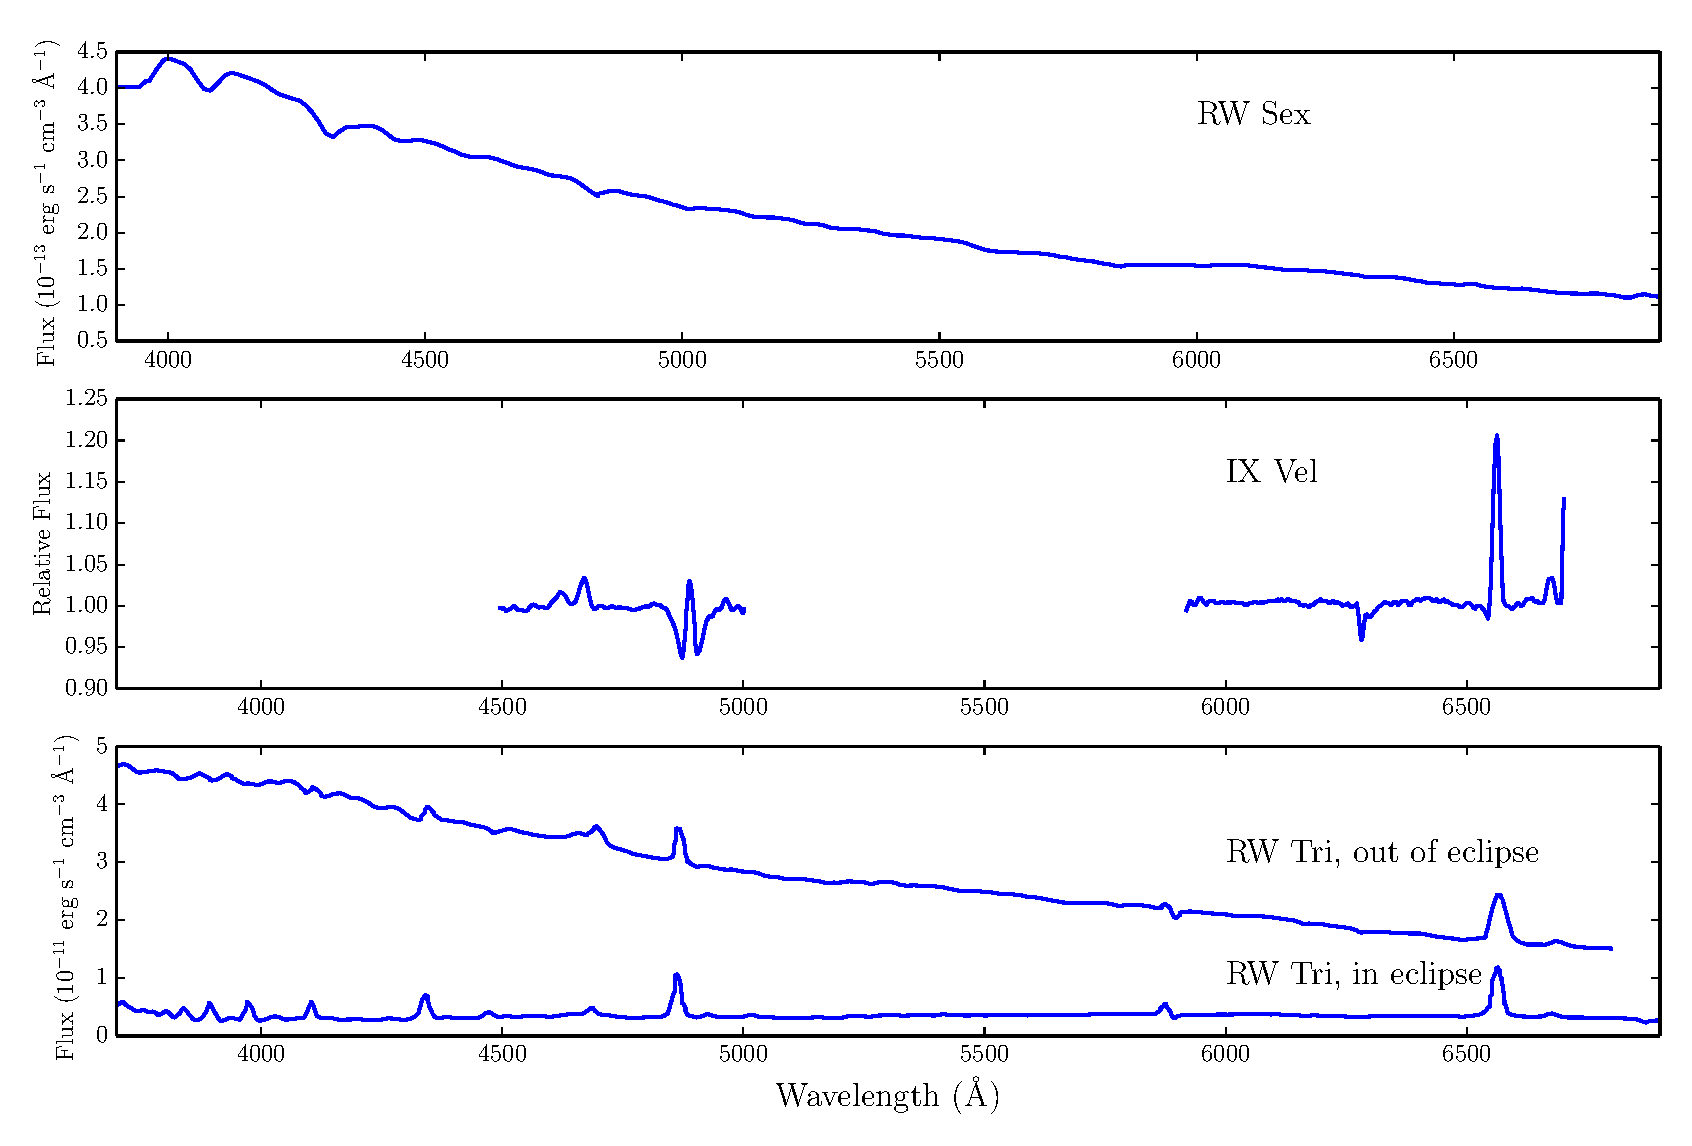
\includegraphics[width=0.5\textwidth]{figures/fig1.eps}
\caption{Cartoon illustrating the three broad classes of sightline discussed in the text.}
\label{cartoon}
\end{figure}


\begin{itemize}
\item Velocity law, kinematics, etc. 
\item Refer to figure 2
\item define velocity law: As in LK02, we follow the prescription of SV93 in both our fundamental biconical wind model and velocity law. 
The poloidal velocity, $v_l$, along a streamline in our model is given
by 
\begin{equation}
v_l=v_0+\left[v_{\infty}(r_0)-v_0\right]\frac{\left(l/R_v\right)^{\alpha}}{\left(l/R_v\right)^{\alpha}+1},
\label{v_law}
\end{equation}
where $l$ is distance measured along a poloidal streamline. This
power-law velocity profile was adopted by SV93 in order to give a 
continuous variation in the derivative of the velocity and a 
ralistic spread of Doppler-shifted frequencies in the outer portion
of the wind (${l > R_v})$. We have similar requirements.
\end{itemize}

% The initial poloidal velocity of the wind, $v_0$ is (somewhat
% arbitrarily) set to $6~\rm{km~s^{-1}}$ for all streamlines, comparable
% to the sound speed in the disk photosphere. The
% wind then speeds up on a characteristic scale length $R_v$, 
% defined as the position along the poloidal streamline at which the
% wind reaches half its terminal velocity, $v_{\infty}$.
% The terminal poloidal velocity along each streamline is set to a fixed
% multiple of the escape velocity at the streamline foot point, 
% \begin{equation}
% v_{\infty}=fv_{esc},
% \label{v_infty}
% \end{equation}
% so the
% innermost streamlines reach the highest velocities.
% The power-law index $\alpha$ controls the shape of the velocity
% law: as $\alpha$ increases, the acceleration is increasingly
% concentrated around $l = R_v$ along each streamline. 
% For large $\alpha$, the initial poloidal velocity
% stays low near the disk and then increases quickly through $R_v$ to 
% values near $v_\infty$. 

% Table~\ref{wind_param} shows the parameters used in the wind model, and Figure~\ref{cartoon}
% shows a sketch of the geometry of our model, with the key parameters labeled.

\begin{table}
\centering
\begin{tabular}{p{3cm}p{4cm}}
\hline Free Parameters 	&	 Value \\ 
\hline \hline 
$M_{WD}$ 	 &	 $0.8 M_{\odot}$ \\ 
$\dot{M}_{acc}$ 	 &	 $3.16\times 10^{-9}~M_{\odot}yr^{-1}$\\ 
$\dot{M}_{wind}$  &	$3.16\times 10^{-8}~M_{\odot}yr^{-1}$\\ 
$r_{min}$ 	&	 $4 R_{WD}$\\ 
$r_{max}$ 	&	 $12 R_{WD}$ \\ 
$\theta_{min}$ 	&	 $20.0^{\circ}$ \\ 
$\theta_{max}$ 	&	 $65.0^{\circ}$ \\ 
$\lambda$ 	&	 $0$ \\ 
$v_{\infty}$ 	&	 $3v_{esc}$ \\ 
$R_v$ 	        &	 $7\times10^{11}$cm \\ 
$\alpha$ 	&	 $1.5$ \\
\end{tabular}
\centering
\caption{Wind geometry parameters used in the benchmark CV model.}
\label{wind_param}
\end{table}

\subsection{Photon Sources}

Identify the photon sources in the model.

\subsubsection{Disk Treatment}
How we treat the disk and why. Refer to LK02, Kurucz, Wade, Murray and Chiang.
% \py has has some flexibility when treating the accretion disk as a source of photons, in which the disk is broken down into annuli 
% such that each annulus contributes an equal amount to the bolometric luminosity. Each annulus can 
% be treated either as a blackbody with the corresponding temperature or as a Kurucz stellar atmosphere model (REF)
% with the appropriate surface gravity and temperature. Both of these methods have flaws. It is known
% from studies of CV accretion disks that they exhibit absorption cores, which can inpact the overall spectrum 
% even if a wind is present (REF), so the blackbody treatment is not complete. However, the stellar atmosphere
% models also have problems \cite{wadedisk}, and there are clear inconsistencies with using a stellar atmosphere beneath a dense
% wind region which itself goes some way to simulating the disk atmosphere. Here we use the Kurucz models,
% partly because they provide the most pessimistic prediction due to the strong absorption beyong the Balmer edge, 
% which is required to be filled in by the recombination emission in the wind (see Section~\ref{balmerjump}).

\subsubsection{Boundary Layer}
Whether we include one, why why not, referring to He II and ionization.


\newpage
%%%%%%%%%%%%%%%%%%%%%%%%%%%%%%%%%%%%%%
%
%          CODE
%
%%%%%%%%%%%%%%%%%%%%%%%%%%%%%%%%%%%%%%%

\section{Radiative Transfer \& Code Validation}

Introduction and description of Python. 

\begin{itemize}
\item Brief, mainly referring to LK02 and H13. 
\item Give a little history to the code. How it improves on e.g. SV93.
\end{itemize}
% \py is a Monte Carlo radiative transfer code which uses the Sobolev approximation.  
% It expands on the work of SV93 and also incorporates techniques described by
% Lucy (1999a, 1999b, 2002, 2003). The code is first described by Long \& Knigge (2002),
% who synthesized the UV spectra of CVs, successfully reproducing P-Cygni resonance line profiles
% whilst solving self-consistently for the thermal balance and ionization structure in the wind
% according to the method of Mazzali \& Lucy (1993). \py has since been used with application
% to QSO wind modeling \citep{higginbottom2013}, which involved a new ionization scheme to deal with the
% more complex power-law spectrum, and encorporation os processes such as Compton scattering in order
% to correctly treat X-ray radiation transfer. In addition, \citep{simmacro2005} modeled
% Brackett and Pfund line profiles in YSOs using \py, using the macro atom scheme outlined by Lucy (2002, 2003) applied
% to a Hydrogen-only model.

% Here, we 
% model the UV resonance lines in much the same way as LK02, using the 
% fast two-level atom approximation which is appropriate for treating transitions with strong
% coupling to the ground state. However, our model has one crucial difference to LK02, as we use
% the macro atom scheme in tandem with this method. Hydrogen and Helium are treated
% as macro atoms in an attempt to provide a better treatment of optical recombination lines (e.g. the Balmer series, He II 4686, He I lines),
% Lyman-$\alpha$, and the recombination continuum which is suspected to play a key role in `filling-in' the Balmer
% photoionization edge (see e.g. Knigge \& Drew 1998). 

\subsection{Ionization scheme}
Description of ML93 ionization scheme and motivation for using it. 

\begin{itemize}
\item First, the SED can be approximated well by a Blackbody due to the 
absence of an X-ray source, and therefore the blackbody treament is appropriate; 
\item Second, this provides continuity from LK02 and allows us to do a like-for-like comparison

% Although H13 developed a new ionization scheme which approximates the 
% SED in a cell with a broken power law, 
\item Here we follow LK02 in using the
ionization scheme presented by Mazzali \& Lucy (1993), who specifically
present the formula 
\begin{equation}
\frac{n_{j+1} n_e}{n_j} = W [\xi + W(1-\xi)]
\left(\frac{T_e}{T_R}\right)^{1/2}
\left(\frac{n_{j+1}n_e}{n_j}\right)^*_{T_R}, \label{ionization}
\end{equation}
which, in principle, accounts for ionizations from and
recombinations to all levels of an ion. 

\end{itemize}
%In this equation, the last
% (``starred'') term on the right hand side refers to the Saha
% abundances, $W$ is an effective dilution factor, $\xi$ is the
% fraction of recombinations going directly to the ground state, and
% $T_R$ and $T_e$ are the radiation and electron temperature
% respectively. LK02 provide a full description of our implementation.

% The reason for using this scheme 
% is twofold; First, the SED can be approximated well by a Blackbody due to the 
% absence of an X-ray source, and therefore the blackbody treament is appropriate; 
% Second, this provides continuity from LK02 and allows us to do a like-for-like comparison,
% which is especially useful in assessing the improvement in Hydrogen line emission, and any changes
% that might occur in the ionization stages of the resonance line species such as CIV. 


\subsection{Macro-atoms}

Description of macro atom and why they are so important. Describe the interplay between macro atoms
and simple ions.
% In its standard operating mode, \py uses a two-level atom approximation \cite[see e.g.][]{mihalas} for its treatment of lines. This approximation works well when treating so-called `resonance lines' (such as \civ, O\textsc{vi}), in which the excited electron is strongly coupled to the ground state, but breaks down for more complex situations such as recombination cascades. To properly model recombination lines, including the Lyman and Balmer series, a more complete treatment of line transfer is required.

% Lucy (2002, 2003\nocite{lucy2002, lucy2003}; hereafter L02, L03) showed that by quantising matter into `macro-atoms', and radiant and kinetic energy into energy packets, it is possible to asymptotically reproduce the emisssivity of a gas in statistical equilibrium without simplifying line transfer. Macro-atoms are finite volume elements with internal transition probabilities that are `activated' by packets of radiant (r-packets) or kinetic (k-packets) energy. A typical activation and deactivation sequence is shown in figure~\ref{macro}.
% A full description is far beyond the scope of this report- consult L02 and L03. 

% The macro-atom scheme has been used with \py before, in a Hydrogen-only mode with application to YSOs \citep{simmacro2005}, but has not yet been applied to AGN or CV problems. With some improvements, the current scheme will enable \py to model H and He recombination lines, for example. The fast, simple treatment of resonance lines 
% can be retained, as the \py implementation allows for non-macro atom treatment for certain ions.

\subsection{Atomic Data}
Description of atomic data used (that is different from H13).
\begin{itemize}
\item Clearly identify and cite sources. 
\item Discuss any limitations and what motivated the level choices in particular 
(i.e. why do we split up he I but not He II, l-mixing, etc).
\end{itemize}

% Atomic data is obtained from the same sources described in LK02 and updated in H13. 
% The additional level and line information required to treat Helium as macro atom was 
% obtained from \textsc{Topbase} \citep{topbase2005}. We treat Hydrogen as a 20-level atom as in S05, where 
% each level is defined by the principal quantum number n, which is appropriate due to
% the degeneracy of each level in the Hydrogen atom. Helium II is treated in much the same way,
% with 10 levels, but He I has larger energy differentials between different l subshells
% and triplet and singlet states. Thus, we still include levels up to n=10 but explicitly 
% treat the l-subshells as distinct levels instead of assuming they are perfectly `l-mixed',
% which will have the pleasant side effect having the potential to produce triplet lines.



\subsection{Code Validation and Testing}


\subsubsection{Non-LTE Level Populations}

Discussion of how we tested the macro atom scheme
\begin{itemize}
\item Figure 2 Case A and B comparisons with Seaton 1959. 
\item I'd possibly also like to include a Helium test w/ ChiantiPy or similar 
\item or maybe TARDIS?
\end{itemize}
% Before proceeding with modeling of CV systems, we need to be sure that our scheme fulfils Lucy's (2002) 
% statement that it will `asymptotically reproduce the emissivity of a gas in statistical equilibrium'.
% For our tests, we use a Hydrogen only `thin shell' mode in \py, in which a single macro atom is created as a spherical 
% shell with a thickness of 1cm. We construct the situation such that all opacities other than 
% bound-free absorption are negligible, and the only cooling process available to the gas is that of
% recombination line emission. This is a mathematical pathology, commonly known as `Case A', and allows
% us to test against analytical calculations.

% As \py normally models dense environments, it assumes each principal quantum number level is
% well `l-mixed' - that is each subshell of a given level is populated according to statistical weight by
% inelastic collisions. It is therefore not possible to compare with non-L mixed calculations such as 
% those presented in Osterbrock (1989\nocite{oster}). Seaton (1959; S59\nocite{seaton}) carried out calculations
% for Case A in the l-mixed case, and is thus a better comparison. Figure 1 shows a comparison between S59
% and \py, showing excellent agreement. Figure 2 shows the Case B comparison, in which the escape probabilities
% for the Lyman lines have been explicitly zeroed.

\begin{figure}[!h]
\centering

\includegraphics[width=0.5\textwidth]{figures/seaton_emissiv.png}
\caption{Case A \& B comparison between S59 and \py at 10000K and 20000K}
\label{seaton}
\end{figure}

%\begin{figure}
%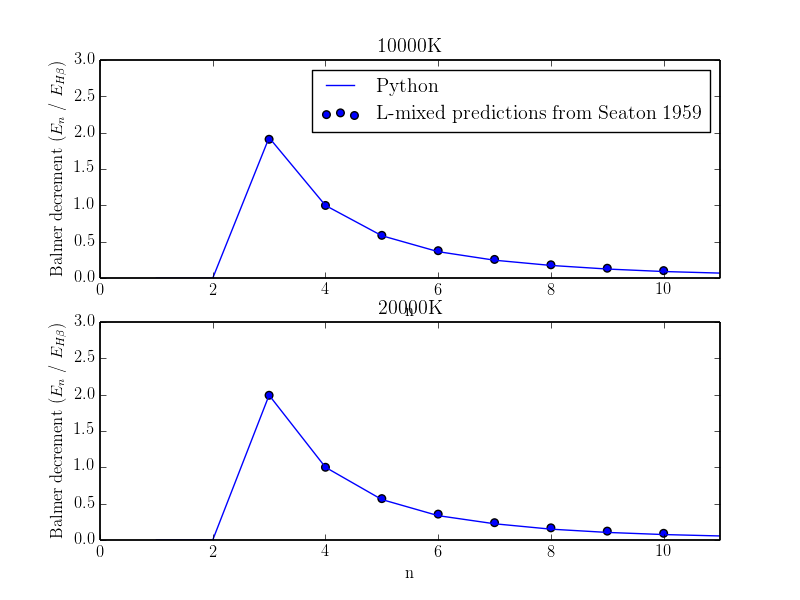
\includegraphics[width=0.5\textwidth]{figures/caseA.png}
%\caption{Case A comparison between S59 and \py at 10000K and 20000K}
%\end{figure}

%\begin{figure}
%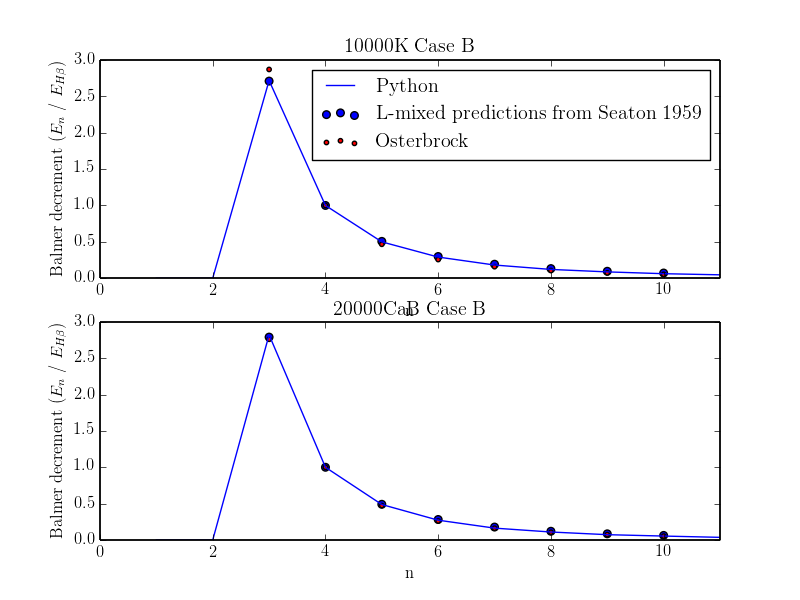
\includegraphics[width=0.5\textwidth]{figures/caseB.png}
%\caption{Case B comparison between S59 and \py at 10000K and 20000K}
%\end{figure}

% This test verifies the treatment of recombination lines in Hydrogen only models, but it is also necessary to test the implementation
% of macro-atoms when other elements are treated as so-called `simple ions'. In this mode, the user can select which species to treat as
% macro atoms, meaning that the other species are still treated with a two-level approximation. This means that the fast treatment of
% resonance lines can be maintained without sacrificing the necessity that all energy packets are indivisible. It is important to verify that 
% this still produces the correct ionization state for the wind. We can test this by comparing against both {\textsc Cloudy} and LK02.

% Figure 3 shows a comparison between the macro atom mode and standard mode of the code using the SV93 model. The ionization state is remarkably similar.



\subsubsection{Ionization}

How ML93 + macro atom hybrid ionization has been tested.

\begin{itemize}
\item Description of past tests: TARDIS, LK02 v Cloudy, NSH v Cloudy.
\item  My own cloudy test with Hydrogen and Helium?
\item  Refer to ionization state sections. 
\item Show in Figure 3- Ion fractions of Helium, Carbon, Oxygen?
\end{itemize}


\begin{figure}[!h]
\centering
\includegraphics[width=0.5\textwidth]{figures/screen.png}
\caption{CLOUDY TEST. Show three panel figure showing Carbon, Helium and Oxygen.}
\label{ions}
\end{figure}

% LK02 presented comparisons of between \py and the widely used photoionization code Cloudy, showing good agreement 
% of calculated ion fractions between the code. In addition, \cite{tardis} present a code for 
% spectral synthesis of Supernova (\textsc{TARDIS}) which compares spectra from a homologous spherical model with
% the ML92 ionization scheme. We are therefore confident that our treatment for so-called `simple ions' is correct.

% To verify that the macro atom treatment is correct, it is important to compare level population tests 
% fro Hydrogen and Helium with that expected from literature. In addition, we check that the dual macro atom/simple ion
% implementation still shows good agreement with Cloudy.

\newpage
\bigskip
\bigskip

%%%%%%%%%%%%%%%%%%%%%%%%%%%%%%%%%%%%%%
%
%          RESULTS
%
%%%%%%%%%%%%%%%%%%%%%%%%%%%%%%%%%%%%%%%

\section{Results}

\subsection{Synthetic Spectra}
Present the spectra with a brief description, .

\begin{figure}
\includegraphics[width=\textwidth]{figures/smplot.pdf}
\caption{Synthetic Spectra computed for sightlines of 22.5, 25, 62.5 and 80 degrees.}
\end{figure}

\subsection{Ionization State}
Present the ionization state with wind plots showing dominant ions.

\begin{figure}
\includegraphics[width=\textwidth]{figures/ionplot1.jpg}
\caption{Synthetic Spectra computed for sightlines of 22.5, 25, 62.5 and 80 degrees.}
\end{figure}



\newpage
%%%%%%%%%%%%%%%%%%%%%%%%%%%%%%%%%%%%%%
%
%          DISCUSSION
%
%%%%%%%%%%%%%%%%%%%%%%%%%%%%%%%%%%%%%%%

\section{Discussion of Results}

\subsection{The Balmer Series}
\begin{itemize}
\item A main result: that we are able to produce the Balmer lines. Comparison to old model without macro atoms?
\item How this changes with inclination
\item Comparison to literature
\item trends along the series, strengths and double v single peaked emission
\end{itemize}



\subsection{The Balmer Jump}
\label{balmerjump}
\begin{itemize}
\item A main result: that we are able to fill in the Balmer jump with the recombination continuum from the wind
\item How this changes with inclination
\item Comparison to literature
\item Discussion of disk atmosphere treatment and its effect.
\end{itemize}




\subsection{Helium Lines}
Discussion of Helium lines in the spectrum.
\begin{itemize}
\item He II 4686, He II 1640 strengths
\item Make the prediction that if 4686 is strong we might expect strong He II 3202 5->3. 
\item Discuss why it wouldn't have been seen yet (spectral coverage)
\item Helium I lines
\end{itemize}



\subsection{UV Resonance Lines}
Compare spectra to LK02 and other models. Are the spectral features preserved, has anything significant changed.
Lyman alpha?

\subsubsection{OVI and the Auger effect}
\begin{itemize}
\item Why it is important
\item how it could be implemented.
\end{itemize}

\subsubsection{The Line Force}
\begin{itemize}
\item Can this wind be radiatively driven? 
\item Why/why not?
\item Figure showing line force throughout the wind as a fraction of some critical value?
\end{itemize}


\newpage

%%%%%%%%%%%%%%%%%%%%%%%%%%%%%%%%%%%%%%
%
%          Comparison with real spectra
%
%%%%%%%%%%%%%%%%%%%%%%%%%%%%%%%%%%%%%%%

\section{Comparison with Data}

Here we compare Python to real data. Hopefully from e.g. a high inclination 
nova like with a number of features which are similar. Discuss the 
similarities and differences and why.

\begin{figure}[!h]
\includegraphics[width=1.0\textwidth]{figures/sd.png}
\caption{Comparison between our benchmark model viewed at xx degrees with the 
non-magnetic Nova Like UX UMa.}
\end{figure}





\newpage
%%%%%%%%%%%%%%%%%%%%%%%%%%%%%%%%%%%%%%
%
%          Conclusions and Future Work
%
%%%%%%%%%%%%%%%%%%%%%%%%%%%%%%%%%%%%%%%


\section{Conclusions and Future Work}

%% Balmer jump


\subsection{Future Work}

In addition to this project, we plan to apply the macro atom scheme to QSOs in order to build on the work of Higginbottom et al. (2013),
in which a benchmark biconical disk wind model was presented. In particular, we hope that the macro-atom scheme will enable the
model to produce significant Lyman-$\alpha$ emission, as is observed in QSOs.


\subsection*{Acknowledgements}
%The work of NH, JHM and CK is supported by the Science and Technology Facilities Council (STFC), via studentships and a consolidated grant, respectively. In particular, we would like to thank Juan Hernandez Santisteban for useful conversations, and for his help extracting SDSS spectra. 
%The authors acknowledge the use of the IRIDIS High Performance Computing Facility, and associated support services at the University of Southampton, in the completion of this work.



\bibliography{mybib.bib}

\end{document}
